\documentclass[11pt,twoside]{book}

\usepackage{geometry}
\usepackage[parfill]{parskip}
\usepackage{graphicx}
\usepackage{amssymb}
\usepackage{pdflscape}
\usepackage{epstopdf}
\usepackage{natbib}
\usepackage{makeidx}
\usepackage{glossaries}

\title{The Development of a Computerized Interactive Teaching Assistant for Purdue's Computerized Homework in Physics\\[0.2in]The CITA on CHIP Project}
\author{Author: Cyrus Vandrevala\\[0.2in]
Co-Adviser: Dr. Andrew Hirsch\\
Co-Adviser: Dr. Lynn Bryann\\
Committee Member: Dr. Laura Pyrak-Nolte\\
Committee Member: Dr. Hisao Nakanishi}

\makeglossaries
\makeindex

\setacronymstyle{long-short}
\loadglsentries{backmatter/glossary}

\begin{document}

\frontmatter
\maketitle
\tableofcontents
\listoffigures
\listoftables
\chapter[Dedication]{Dedication}

\begin{flushright}
I would like to thank my family for their support and encouragement - my dad for the inspiration to pursue a higher degree, my mom for her compassion and delicious food, my brother for his calming presence, and my sister-in-law for commiserating with me during the tough times.

I would especially like to thank my wife for her support. She stuck with me throughout my entire graduate career, during all of my ups and downs. If that's not love, I don't know what is.
\end{flushright}
\chapter[Abstract]{Abstract}

\chapter[Acknowledgements]{Acknowledgements}

I would like to thank Dr. Rebecca Lindell and her research group for their guidance throughout the project.

I would also like to thank Dr. Joe Redish, Dr. Ruth Chabay, and Dr. Bruce Sherwood for their input. Talking with them helped set this project in motion.

\mainmatter
\chapter[Introduction]{Introduction}

\section{Background}

Due to the increased popularity of online classes and the rising enrollment in foundational science and \index{engineering}engineering courses, professors and teaching assistants are under constant pressure to provide students with the assistance that they need throughout the semester - especially on homework assignments. When direct help from a faculty member is not available, students need an interactive learning tool that guides them through homework problems. This is especially important in an environment where nontraditional students with diverse schedules must attend class\cite{choy2002, horn1996}. Student success in any course requires good communication betthe research teamen students and instructors. Hothe research teamver, the expectation of access to faculty at any time is unrealistic with all of the duties of the teaching staff.

We are developing a \gls{cita} for the calculus-based introductory electricity and magnetism course for engineers at Purdue University. This program will guide students through homework problems while teaching the nuanced techniques of physics problem solving. The most often heard statement from students attempting a physics problem is, ``I don’t even know where to begin.'' Our goal is to design an interactive component for every homework problem that will develop help students generate an understanding of physics concepts and enchance their problem solving skills.

Most computerized homework systems only provide a ``correct'' or ``incorrect'' response to an ansthe research teamr. If a student receives the ``incorrect'' message, there is no explanation as to why their logic was wrong. Even worse, these systems do not provide instruction on how to proceed from the point at which the student made a mistake. Sometimes, there is a link to a passage in the textbook that lists the derivation of the problem without specific context. At this point, the student either has to email an instructor, wait for recitation later in the the research teamek, or seek special appointments with instructors. Thus, the learning process is interrupted as the student waits for simple guidance. Our goal is to design, develop, implement, and analyze an online system that is available at any time to provide focused guidance to help students acquire the knowledge and skills necessary to solve the problem.

\section{Overview of Electricity and Optics at Purdue}

This study takes place in PHYS 24100 and PHYS 24100D (Electricity and Optics) which are the introductory electromagnetism courses for \index{engineering}engineering majors at Purdue University (with the exception of the electrical engineering majors who take PHYS 27200). The ``D'' represents that it is a distance learning course (i.e. an online course). The content in these two classes is exactly the same; they only differ in the fact that the distance learning sections watch video lectures and attend live online recitations through Cisco WebEx while the regular sections watch live lectures and attend live recitations on campus.

Electricity and Optics is generally taken after students complete PHYS 17200 - Modern Mechanics. This introductory mechanics course is currently taught using the Matter and Interactions textbook by Dr. Ruth Chabay and Dr. Bruce Sherwood\cite{chabay2010}. PHYS 24100 or PHYS 24100D is a prerequisite for many of the intermediate \index{engineering}engineering courses at Purdue University.

Engineering students usually take this course in the fall semester (the ``on-semester''). Alternatively, some students choose to take the course in the spring or summer due to the fact that they are either ahead or behind in their schedules (the ``off-semesters''). Figure \ref{fig:enrollment} shows the total enrollment in PHYS 24100 and PHYS 24100D over the last three years. Note that PHYS 24100D was not created until summer 2012.

Figure \ref{fig:percent} shows the percent of the total class that is enrolled in the distance learning section of Electricity and Optics. It is important to note that although the research team try to separate the online and on-campus sections, the placement is dependent on student preference. For example, during the summer semester in 2015, the research team had such a high demand for online courses that the research team decided to combine all of the sections into PHYS 24100 rather than separating them into PHYS 24100 and PHYS 24100D. Data is not shown in figure \ref{fig:percent} for the year 2015 since it is as of yet incomplete.

\begin{figure}[!hb]
	\centering
	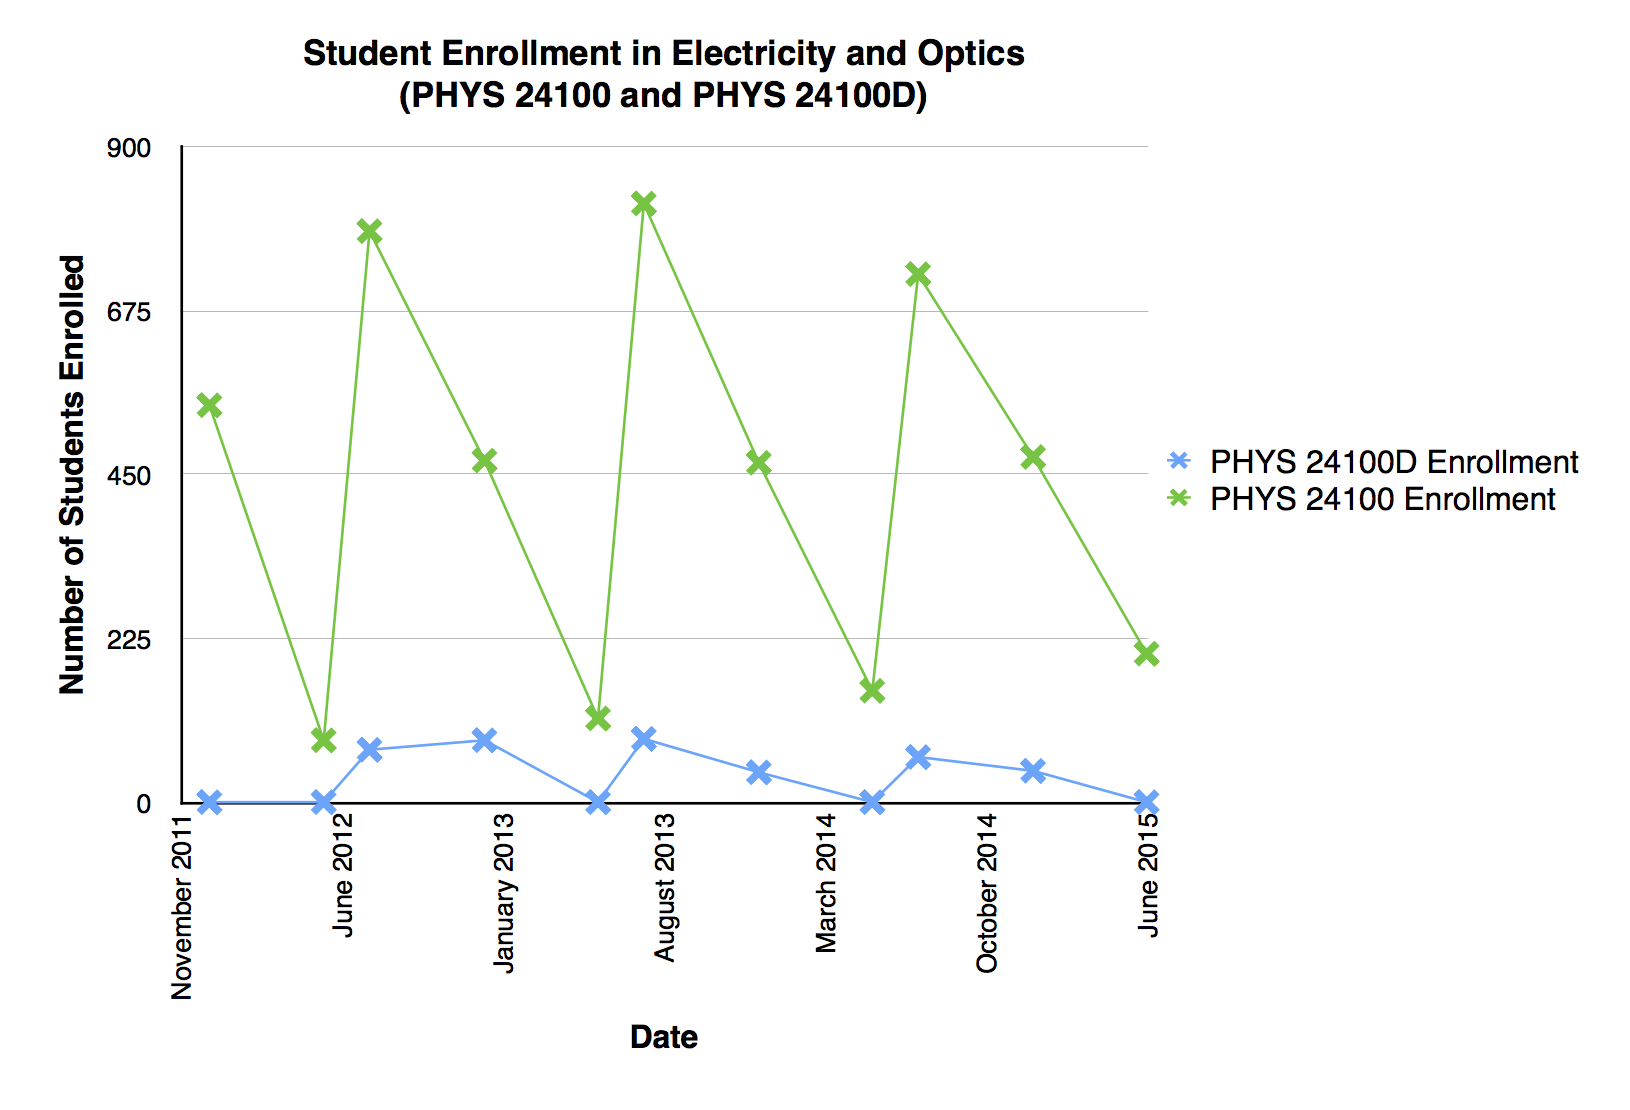
\includegraphics[width=5in]{img/chapter1/enrollment}
	\caption[Enrollment in PHYS 24100 and PHYS 24100D Over the Last Three Years]{Enrollment in PHYS 24100 and PHYS 24100D Over the Last Three Years}
	\label{fig:enrollment}
\end{figure}

% ^Redo this chart^

\begin{figure}[!hb]
	\centering
	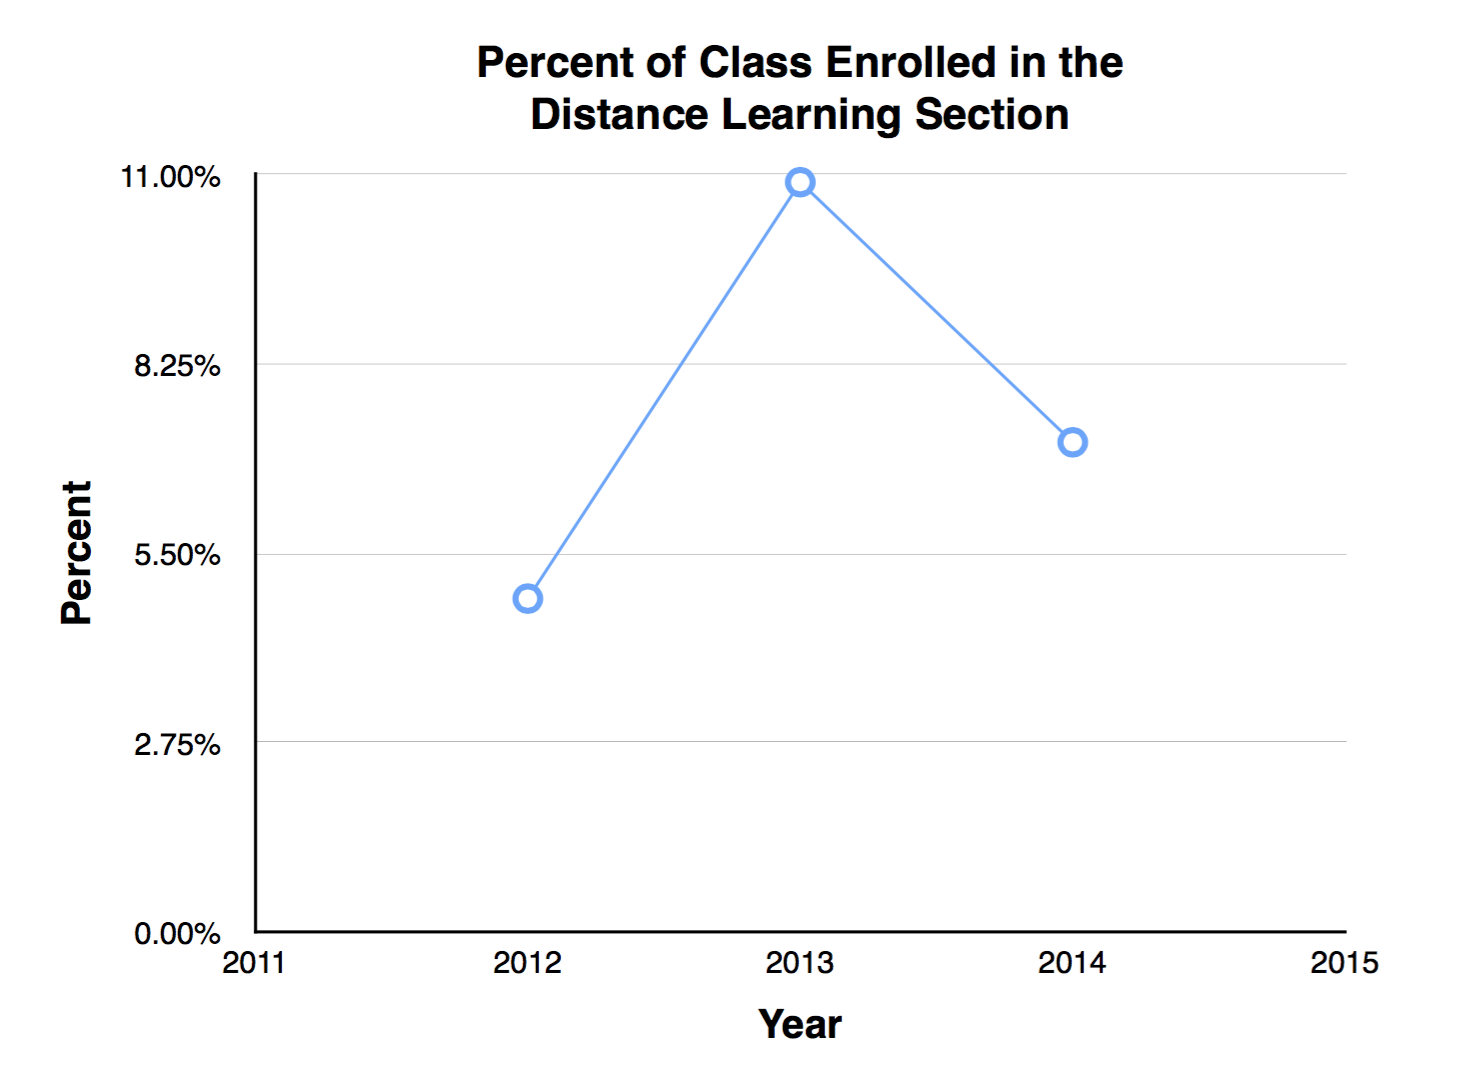
\includegraphics[width=5in]{img/chapter1/percent}
	\caption[Percent of Students in PHYS 24100D (Distance Learning)]{Percent of Students in PHYS 24100D (Distance Learning)}
	\label{fig:percent}
\end{figure}

\section{Overview of Homework in Electricity and Optics}

PHYS 24100 and PHYS 24100D use an in-house homework system called \gls{chip}. The \gls{chip} system is based on the CPlite homework system from the \gls{uiuc}. Purdue University adopted an early version of CPlite in 1997 and continued to make improvements to it over the next decade, adding statistical analysis tools, gradebooks, and updated homework problems. \gls{chip} services not only the introductory electromagnetism courses, but also many of the other physics courses at Purdue University.

\subsection*{Strengths}

\gls{chip} is a the research teamll established system that has over a decade of in-the-field use. One of its biggest advantages is that it has no ties to any external companies or organizations. Faculty members at Purdue are free to recommend updates or modify the source code as they wish. (Rephrase this)

All of the \gls{chip} servers are maintained on Purdue University campus in the physics building by the university's support team. \gls{chip} has a dedicated staff of experts that run and maintain the system; this includes technology professionals who maintain the stability and security of the system as a whole and faculty members who use it to assign and grade homework. No aspect of \gls{chip} has to be outsourced to a third party. One huge advantage of this is when students ask questions or send error reports, they are talking directly with a course instructor rather than a secondary source.

\gls{chip} has a the research teamll developed database of problems from a variety of textbooks. These problems are free to use and modify, as long as the changes are contained within \gls{chip} software. Thus, the physics classes at Purdue have ready access to hundreds of potential homework, quiz, and exam questions.

\gls{chip} has the framework in place to collect statistics on student performance during the semester. On a basic level, it is capable of recording student scores in a variety of assignments. Hothe research teamver, it can also perform a basic statistical analysis - generating histograms, filtering data, and comparing student scores against a baseline. Since \gls{chip} keeps a secure archive of scores from previous semesters, this data can be used to analyze the progress of a class.

\subsection*{Weaknesses}

Although \gls{chip} has a successful history at Purdue, it is not without its problems. The \gls{chip} program was coded just as the internet was beginning to receive mainstream acceptance. Thus, while the \gls{gui} was revolutionary at one time, it has begun to show its age. The overall look and layout of \gls{chip} has not kept up with modern devices. Specifically, \gls{chip} buttons and menus do not render the research teamll on small screens like cell phones, tablets, and netbooks.

\gls{chip} has a lot of underutilized features. For example, although many statistical analysis tools are available on the system, they are rarely used due to the fact that they are either hard to find or have a steep learning curve. Another underutilized features of \gls{chip} is the interactive example.

Although \gls{chip} has resources for creating tutorials within homework problems, the vast majority of the homework problems provide no help to students who are struggling. Homework problems can be written as an interactive example and given a linear directory structure under which hints and guides can be placed. The student sees a help menu on the specific homework problem and can choose to be guided through the analysis in a step-by-step fashion. Interactive examples have been implemented on only 29 out of the 139 homework problems that students complete in a semester (about 20.9\% of the problems).

\section{Student Comments}

Student comments in \gls{chip} problem reports and semester evaluations support the need for an interactive tutorial system. Many students comment that the content in the course seems disconnected. Thus, students often think that they are covering many diverse topics, rather than a few key laws.

\begin{quote}
The course goes over a bunch of equations but concepts are not really taught. It is hard to understand the material, I feel as if we are just given equations to memorize without understanding what goes on in the problems we deal with.

- Anonymous Student from Spring 2013
\end{quote}

\begin{quote}
I think the text book has too much unnecessary stuff, I sometimes dont really know which part to focus on, it could be helpful if they told us where to focus on.

- Anonymous Student from Summer 2014
\end{quote}

Many have commented on the need for some sort of tool to help them get through the homework.

\begin{quote}
There should be more helping tools, rather than just completing homework. We should have exams relevant to the homework, or reviews/practice of what to expect.

- Anonymous Student from Fall 2013
\end{quote}

\begin{quote}
have more organized homework

- Anonymous Student from Spring 2014
\end{quote}

\begin{quote}
Having a concept map connecting laws and necessary concepts to each other would be helpful as a resource to students. It's difficult enough trying to see connections as learning, but having concept maps that professors/TAs refer back to will allow the students to build with that knowledge in mind.

- Anonymous Student from Summer 2014
\end{quote}

The interactive examples that we do have make up a small percentage of the total homework. However, they are very popular among students. Every semester, students comment on how helpful these examples are.

\begin{quote}
Thank you for the help section in this problem! It was very well written and helped me figure out the problem and (hopefully) similar ones in the future!
\end{quote}

These examples are representative of the need for a tutorial system in the introductory physics courses. The interactive examples can be expanded to assist the thousands of students enrolled annually in the course.

\section{Statement of Development}

We want to develop \gls{cita} for the second semester of introductory physics (Electricity and Optics). This system would be available to guide students through the homework, not only teaching them physics concepts but also good problem solving skills. The development and implementation of \gls{cita} on \gls{chip} requires work on many fronts:

\begin{enumerate}
\item Converting each traditional homework problem into an interactive example, complete with a tutorial that builds problem solving skills as the research teamll as teaches physics
\item Updating the \gls{gui} on \gls{chip} to make the examples easy to follow
\item Utilizing the unused statistical analysis tools in \gls{chip} in order to track student progress and implement constant improvements
\end{enumerate}

\section{Research Questions}

Once the research team implement the system, the research team wish to ansthe research teamr two questions:

\begin{enumerate}
\item How does the branching structure of our interactive examples influence student learning of content? Normative vs. non-normative conceptions.
\item How does the branching structure of our interactive examples influence student problem solving approaches?
\item What are students perceptions about (define this further a, b, c)?
\end{enumerate}

\chapter[Chapter 2: Theories of Learning]{Theories of Learning}

\section{Background}

\section{Paradigms of Learning}

\subsection{Behaviorist Theories}
\subsection{Cognitivist Theories}
\subsection{Constructivist, Social, and Situational Theories}
\subsection{Motivational and Humanist Theories}
\subsection{Design Theories and Models}
\subsection{Descriptive and Meta Theories}
\subsection{Identity Theotries}
\subsection{Miscellaneous Learning Theories and Models}

\section{My Focused Learning Theory}


http://www.learning-theories.com/

When learning new material students bring with them the prior knowledge that they had of the subject at hand. This knowledge includes both correct models of how the world works as well as incorrect, pre-existing notions of the universe. These pre-existing notions diverge from what the teacher is trying to teach.

Teaching learning gap (Redish and Steinberg 1999)

It is tempting to quantify how ingrained a model is in student's heads. Zeilik and Bisard call deeply ingrained misconceptions that are hard to change structural misconceptions. Alternatively, they call easily changed misconceptions factual misconceptions\cite{zeilik2000}. However, a pre- and post concept inventory showed no difference in gains between these two distinctions. However, even though the data showed no difference, they still found it useful to track misconceptions in order to develop lessons for their courses.

Zeilik et al 1997

I use the advice of Zeilik and  Bisard to track misconceptions\cite{zeilik2000}
If I want to teach as efficiently as possible, I need to target misconceptions.
\chapter[Chapter 3: Research Methodology]{Research Methodology}

\section{Background}

\begin{figure}[hb]
	\centering
	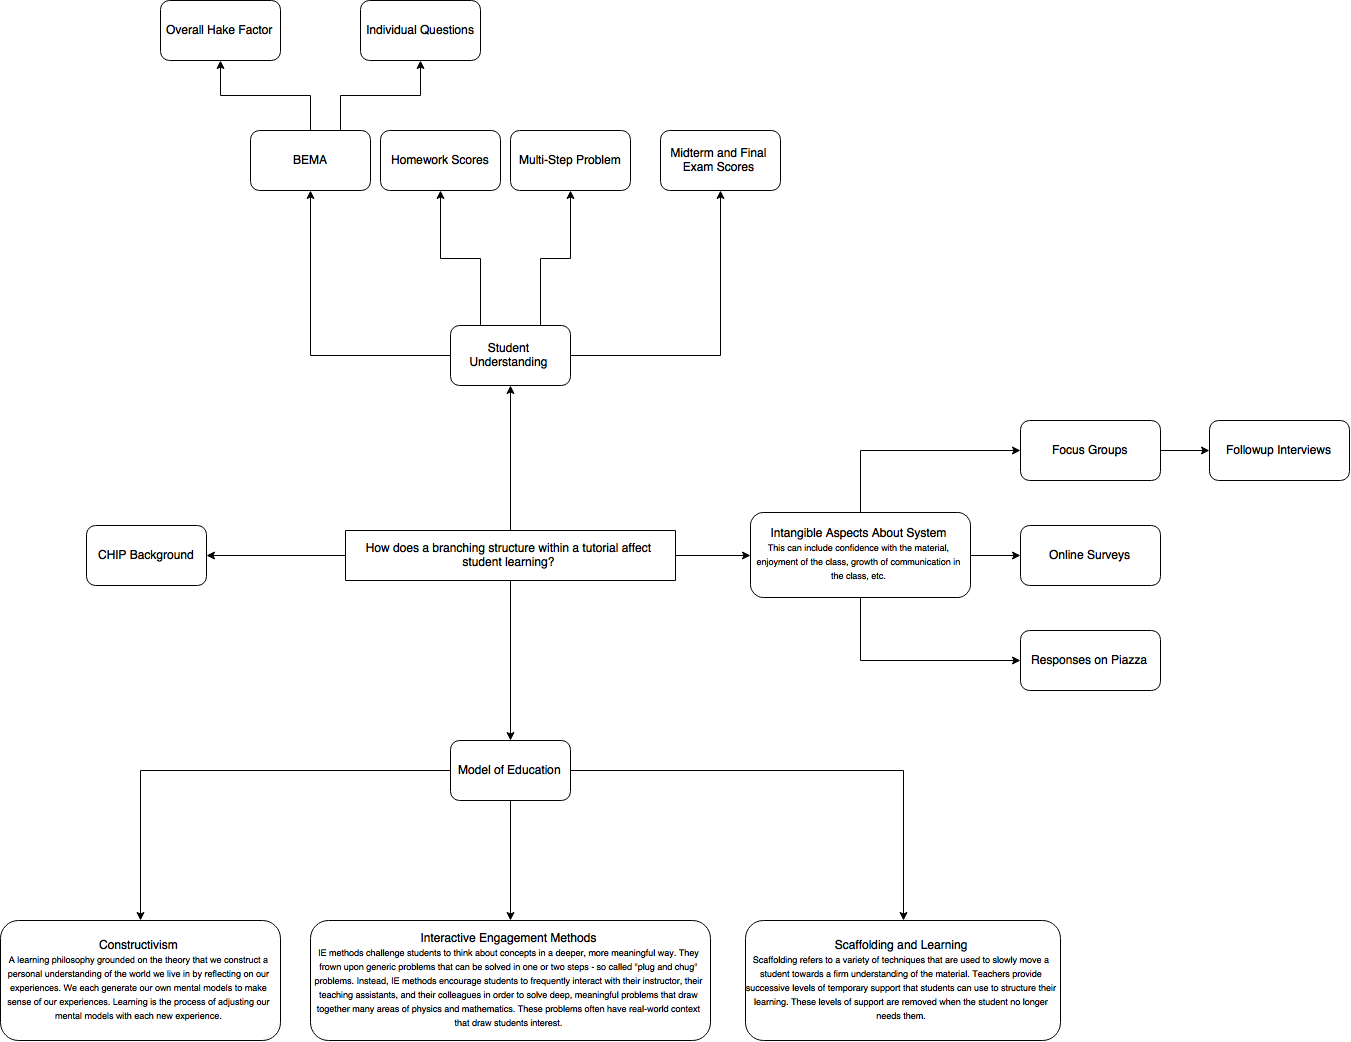
\includegraphics[width=6in]{img/chapter3/flowchart}
	\caption[Flowchart]{Flowchart}
\end{figure}

\subsection{Number of Students Impacted Each Year}

The combined yearly enrollment of PHYS
241 and PHYS 241D has a yearly average
enrollment of 1496 students from science and
engineering. Yearly enrollment in the online
portion of the course (started in Summer 2012)
has been increasing (Figure 2).

\section{Reflexivity}

Our team for the development and implementation of \gls{cita} on \gls{chip} consists of Mr. Cyrus
Vandrevala (who will perform content development and coding to implement \gls{cita} on \gls{chip})
with oversight by Prof. Hisao Nakanishi and Prof. Laura Pyrak-Nolte. Mr. Vandrevala has been
a teaching assistant for PHYS 241 and PHYS 241D since Fall 2011, has coordinated the course
during summer sessions, and was instrumental in the development of the online course videos,
online recitation format, and online forum. Prof. Hisao Nakanishi has taught PHYS 241 and
more importantly is the “father” of \gls{chip}. Professor Nakanishi takes an active role in ongoing
updates and improvements to content, functionality and robustness of the system. He also
addresses student questions sent through \gls{chip}. Professor Laura Pyrak-Nolte has taught PHYS
241 since 2005, coordinated the course since Fall 2011 and is the online lecturer (i.e. in the
online videos) for PHYS 241D.

\section{Exams and Quizzes}



\section{Homework}

The ultimate test of \gls{cita} on \gls{chip} is the ability to solve problems on exams. Student
performance on exam problems that are similar to \gls{cita} enhanced problems will be used to
determine if \gls{cita} improved learning outcomes, i.e. whether or not students have learned
specific problem solving strategies. We can correlate exam scores with:
• Which students use \gls{cita} (“A” students or students at all grade levels)
• When students started using \gls{cita} (before or after first exam, first homework, etc.)
• How many attempts on a problem are made before using \gls{cita}
• How many attempts to solve a problem are needed after using \gls{cita}
• After using \gls{cita} on one problem is it used on every problem
• Comparison of performance on \gls{cita} enhanced practice exams, non-\gls{cita} enhanced
practice exam and the performance on class exams.
In addition, we will use the standard assessment tool BEMA (Brief Electricity and Magnetism
Assessment) developed by Ding et al. (2006) to compare with our metrics. With an average total
yearly enrollment of 1500, sufficient statistics will be generated to determine the impact of \gls{cita}
on student learning

\section{Concept Assessment Instruments}

Concept inventories and assessment instruments are a useful method of assessing student knowledge of the material; however, they are not simply tests that can be quickly put together and administered year after year. Lindell and Ding describe how it takes years to determine the validity and reliability of the results of a given concept inventory. They describe how reliability (precision) and validity (accuracy) play a role in the inventories and cite how factors such as age, course structure, geography, language, delivery of the tests, and wording of questions can influence the results of the assessment\cite{lindell2012}.

\subsection{Brief Electricity and Magnetism Assessment (BEMA)}

The \gls{bema} was developed by Ruth Chabay, Bruce Sherwood, and Fred Reif in 1997. Although it was originally designed to measure student retention of electricity and magnetism concepts three months to five semesters after completing an introductory electricity and magnetism course, it is now often used to analyze student learning between the beginning and end of the semester. It is a useful tool to assess the understanding of electricity and magnetism concepts that are covered in a college-level calculus-based introductory physics course\cite{ding2006}.

The \gls{bema} is a multiple choice test consisting of qualitative questions and a few simple calculations. Lin Ding et al. performed an analysis of the \gls{bema}, showing that it is a reliable assessment tool for introductory electricity and magnetism courses\cite{ding2006}. We use the \gls{bema} extensively in our research to analyze student's understanding of the course material.

\subsection{Force Concept Inventory}

The \gls{fci}􏰁 is a multiple choice test that is used to measure a student's understanding of introductory mechanics. It is given at the beginning of an introductory mechanics course as a pre-test and again at the end of the course as a post-test. The pool of answers on the test are designed to correspond to common student misconceptions of mechanics; they were developed through a series of student interviews\cite{hestenes1992}.

Coletta et al. have observed a strong correlation between the normalized gain on the \gls{fci} and SAT scores. They go so far as to state that SAT scores might be a good indicator of the expected normalized gains within a classroom\cite{coletta2007}.

\section{Other Methods}

\section{Numerical Measures}

\subsection{Hake Factor (Gain Index)}

Normalized gain (G) vs. normalized gain <g>

\subsection{Gender Gap}

What am I trying to improve? What should I test?
Test scores -> Assess using PHYS 241 exam grades
Homework scores -> Assess using PHYS 241 homework grades
Quiz grades -> Assess using PHYS 241 quiz grades
Overall grades -> Assess using PHYS 241 course grades
Knowledge of qualitative electromagnetism concepts -> Assess using BEMA
Problem solving strategy -> Assess using worked out problems with custom rubrics
Student enjoyment in physics -> Personal interviews and class surveys
Student confidence in problem solving -> Personal interviews, worked out problems, and class surveys
Ability to make predictions in new and novel situations -> Give students advanced problems that they need to categorize
Ability to create diagrams -> Custom problems, draw a diagram from written directions
Ability to teach a concept -> Have them reteach the concept using a custom rubric
Close the gap between genders -> Test each gender and see if the gap closes
Close the gap between socioeconomic groups -> Test each group and see if the gap closes
Catch US students up to foreign students -> Test each group and see if the gap closes
Perform better in the lab (physical experiments) -> Create a lab assessment, maybe between 172 and 241
“Thinking like a physicist” -> Videotape how students solve interesting problems
The BEMA might not be a good way to assess \gls{cita}
Consider worked out problems
Track how far students get into problem using a custom rubric
Perhaps this can be implemented during recitation
Bruce and Ruth have a great presentation on their site as a demonstration

\section{Budget}

We are requesting support for graduate student, Mr. Vandrevala, for two years to perform the work to achieve of objective of creating \gls{cita} on \gls{chip}. In addition, funds for supplies for research materials, electronic equipment and software are also requested. Funding is also requested for travel for Mr. Vandrevala to attend education conferences to present our work. The budget is given in Table 1 for a project period of two years (1/1/2015 – 12/31/2016).

\section{Privacy}

It is important to protect student records when doing a study like this. All records will be stored on \gls{chip} servers, maintained on Purdue campus.

We will only analyze data after the semester has ended. This will ensure no conflict of interest between the study and student grades. Interviews might have to take place during the semester due to scheduling. However, the participants will be anonymized in order to protect their identity.

Additionally, all interviews and focus groups will identify participants with letters or numbers rather than names (participant A, B, C, etc.). This includes recordings and transcripts.

\section{Development and Analysis Timeline}

The timeline for the development, implementation and assessment of \gls{cita} on \gls{chip} is shown in Figure 1. In Spring 2015, the \gls{gui} will be updated for instructors and students, the assessment tools will be tuned to included monitoring the impact of \gls{cita}, and \gls{cita} enabled problems will be added in preparation for the summer courses. \gls{cita} enabled homework problems will be rolled-out in Summer 2015 and provide important feedback from students and instructors on the ease of use, helpfulness of suggestions, and acquisition of appropriate/necessary learning data needed for assessment. Concurrently, \gls{cita} will be expanded to practice exam problems during Summer 2015 along with any improvements based on initial user feedback. Summer enrollment in 2014 was on the order of 150 students. The next challenge is to test the system in Fall 2015 with projected enrollment between 775 – 800 students. The Fall 2015 student learning data will provide sufficient statistics to begin the assessment and efficacy of \gls{cita} on \gls{chip}. In addition, work will continue on expanding \gls{cita} with more homework problems and exams from Spring 2015 and Summer 2015. Our approach is to continually upgrade \gls{cita} based on student and instructor feedback. At the end of fall 2016, we will meet and assess the impact of \gls{cita} on student learning.

\begin{table}[!ht]
  \centering
  \begin{tabular}{|l|l|l|l|}
    \hline
    \textbf{Date} & \textbf{Events} & \textbf{Notes}\\
	\hline
	Spring 2015 & Create Branching Help Button in \gls{chip} & Spearheaded by Dr. Hisao Nakanishi\\
	& Create \gls{cita} Homework Problems & hi\\
	\hline
	Summer 2015 & Create \gls{cita} Homework Problems & Finish\\
	& Beta Test of \gls{cita} Homework Problems & hi\\
	\hline
	Fall 2015 & Update \gls{gui} for \gls{chip} & Pending\\
	& Update \gls{gui} for \gls{cita} & Pending\\
	& Update Assessment Tools on \gls{chip} & Pending\\
	\hline
	Spring 2016 & Expand \gls{cita} Problems & Pending\\
	& Analyze \gls{cita} Data from Fall 2015 & Pending\\
	Summer 2016 & 2 & 3\\
	Fall 2016 & 2 & 3\\
	& Expand \gls{cita} Problems & Pending\\
	\hline
  \end{tabular}
  \caption{Project Timeline}
  \label{tab:timeline}
\end{table}
\chapter[Chapter 4: Current Progress]{Current Progress}

\section{Background}

Work started on the CITA on CHIP project in earnest in February 2015.

Personalization is important
Analytics and tracking progress
It might be able to better serve women and minorities in STEM
Focus on student’s questions (it promotes individual thinking)
Track progress in an individualized way
Coach students through problems
Consider multiple iterations of the same lesson
Stress problem solving strategies
This program could be an equalizer in the classroom
This program might boost student confidence
This program might be good for international students with poor English
Stress multiple learning mechanisms
Break up each problem into tiny pieces
Provide immediate feedback
This program may help customize the curriculum
It is a non-linear way to solve problems

\section{Analysis Tools}

\subsection{CHIP}

The CHIP program has a set of built in tools.

\subsection{R}

\subsection{Muffin}

Over the course of this project, we will have to deal with data from a variety of sources. For example, we will have to review CSV data from the CHIP website, JSON data from the Piazza website, audio data from focus group transcripts, and written data from notes taken by teaching assistants over the course of the study. We need a simple and efficient way to translate one data format into another so that it can be used with \gls{chip}.

I have written an open-source data analysis toolbox called Muffin that will handle this information. Muffin is a set of Ruby functions that will simply read and write data to a format appropriate for our study. The source code for Muffin is hosted on \index{RubyGems}RubyGems as well as on my personal \index{GitHub}GitHub page.

Muffin is simply a toolbox that converts data from one format to another. It does not store anything or conduct analysis in any way. Thus, privacy is maintained, even when the Muffin source code is freely distributed online.

\section{Development of CITA}

We only continue exploring a topic if we feel comfortable in our environment and we feel it is worth it. We are economic creatures.

Goals
With the increased popularity of the online course as well as increased enrollment in the course as a whole, students need a homework website with an interactive learning tool that guides them through the homework no matter what time of day (i.e. different time zones, work schedules).  We want to design an computerized interactive TA (iTA) that is available at any time.

We want to design interactive components for each individual problem that can help students develop an approach to problem solving.  The CITA will guide students through problems in such a way as to develop critical thinking and problem solving skills.

High school teachers want to take the course to become accredited.  They see how physics should be thought out / structured.

High Priority Goals
- Update all content with \gls{cita} hints
- Update the statistical analysis parts of the site for student learning outcomes (interactive graphs of statistics)
- Review the site and bring all useful components to the forefront

Medium Priority Goals
- Update site graphics
-> Faculty First
-> Students Second
- Update figures (interactive?)

Low Priority Goals
- Blackboard/Canvas/Whatever Integration
- Mobile Support?

\subsection{Shallow CITA}

\index{Shallow CITA}

\subsubsection{Postscripts}

\index{Postscripts}

\subsubsection{Estimation Problems}

\subsection{Immersive CITA}
\subsubsection{None}
\subsubsection{Linear}
\subsubsection{Branching}

\section{What CITA Does Accomplish}

\section{What CITA Does Not Accomplish}

It is important to set boundaries.

\subsection{It Does Not Replace Teachers}

CITA in no way is designed to replace the job of a teacher in the classroom.

\subsection{It is Not a Course Management Tool}



\section{Background}

\section{Building the System}

\subsection{Shallow CITA}

\index{Shallow CITA}Shallow CITA is used to catch all of the ``low-hanging fruit''.

Units
Question Phrasing
Some negative signs (some require more explanation)

\subsection{Immersive CITA}

\subsection{Postscripts}

\section{Research Question and Hypothesis}

\section{Methodology}

\section{Results}

\subsection{Summer 2014 vs. Summer 2015 Homework Scores}

INCLUDE BAR CHART COMPARING SCORES HERE. MAKE SURE THAT THE STANDARD DEVIATIONS ARE INCLUDED. BOX AND WHISKER PLOTS MIGHT ALSO BE APPROPRIATE.

\appendix
\chapter[Demographic Survey]{Demographic Survey}

\section{Background}

This survey was administered to PHYS 24100 students in the first week of the summer 2015 session. If students completed the survey, they received ten bonus points (equal to the weight of one quiz). It was used to collect general demographic data in order to assess the quality of the CITA program and learn about general trends in the course.

\section{Student Demographics Survey}

Please be sure to make an entry for each question before clicking the submit button. Once you submit a choice for a question, your answer cannot be changed for that question. However, if you submit your choices for only some of the questions, you can come back to this survey prior to the deadline and fill out the remainder of the choices later.

What is your class at Purdue?

\begin{enumerate}
	\item Freshman
	\item Sophomore
	\item Junior
	\item Senior
	\item Graduate
	\item Not Listed
\end{enumerate}

Are you on-campus or off-campus this summer?

\begin{enumerate}
	\item On-Campus
	\item Off-Campus
\end{enumerate}

What is your college/school at Purdue?

\begin{enumerate}
	\item Agriculture
	\item Education
	\item Engineering
	\item Exploratory Studies
	\item Health and Human Sciences
	\item Liberal Arts
	\item Management
	\item Pharmacy
	\item Science
	\item Technology
	\item Veterinary Medicine
	\item Not Listed
\end{enumerate}

If you are in the College of Engineering or the College of Science, what is your primary major?

\begin{enumerate}
	\item BIOL
	\item CHM
	\item CS
	\item EAPS
	\item MA
	\item PHYS
	\item STAT
	\item SCI
	\item AAE
	\item ABE
	\item BME
	\item CE
	\item CEM
	\item CHE
	\item ECE
	\item EEE
	\item ENE
	\item ENGR
	\item EPE
	\item IDE
	\item IE
	\item ME
	\item MSE
	\item NUCL
	\item I Am Not in Science or Engineering
\end{enumerate}

Are you a domestic or foreign student? A domestic student is a US citizen, US national, or resident alien of the United States.

\begin{enumerate}
	\item Domestic
	\item Foreign
\end{enumerate}

What is your racial/ethnic classification?

\begin{enumerate}
	\item American Indian or Alaska Native
	\item Asian
	\item Black or African American
	\item Hispanic or Latino
	\item Indian Subcontinent
	\item Native Hawaiian or Other Pacific Islander
	\item White
	\item Multiracial or Biracial
	\item Not Listed
\end{enumerate}

What is your gender?

\begin{enumerate}
	\item Man
	\item Woman
	\item Transgender
	\item Not Listed
	\item I Prefer Not to Disclose
\end{enumerate}

Is PHYS 24100 required or an elective for you?

\begin{enumerate}
	\item Required by your major/department
	\item Required by your school/university
	\item Elective
\end{enumerate}

If you satisfied the pre-requisite of PHYS 17200 by taking it at Purdue, select the grade you received (options 1-5). If not, select how you satisfied this requirement (options 6-8).

\begin{enumerate}
	\item A
	\item B
	\item C
	\item D
	\item PASS
	\item Physics Test-out Exam
	\item AP Credits
	\item Transfer Credits
\end{enumerate}

If you took PHYS 24100 at Purdue previously, please select the most recent grade that you received.

\begin{enumerate}
	\item A
	\item B
	\item C
	\item D
	\item F
	\item PASS
	\item NOT PASS
	\item I have not taken PHYS 24100
\end{enumerate}

What is your expected grade in this course?

\begin{enumerate}
	\item A
	\item B
	\item C
	\item D
	\item F
	\item PASS
	\item NOT PASS
\end{enumerate}

Did you take an electricity and magnetism course in high school?

\begin{enumerate}
	\item Yes, at a level comparable to PHYS 24100
	\item Yes, at a lower level than PHYS 24100"
	\item No
\end{enumerate}

What is the highest level of Calculus course you have taken and passed? Calc I is the first semester calculus (similar to MA161/165 at Purdue and typically includes plane analytic geometry and introduction to one-variable differential and integral calculus). Calc II is the second semester calculus (similar to MA162/166 and typically includes vectors in two and three dimensions, more integration techniques, various orthogonal coordinate systems, surfaces, etc.). Calc III is the third semester calculus (similar to MA261 and typically multivariate calculus).

\begin{enumerate}
	\item Calc I
	\item Calc II
	\item Calc III or higher
	\item I have never taken calculus
\end{enumerate}

If you took Calc I at Purdue, what grade did you receive in it (options 1-5)? If not, how did you satisfy Calc I (options 6-8)? Calc I is a pre-requisite for Calc II, which is a co-requisite for PHYS241.

\begin{enumerate}
	\item A
	\item B
	\item C
	\item D
	\item PASS
	\item By MA Test-out Exam
	\item By AP credits
	\item By Transfer Credits
	\item I have not satisfied this pre-requisite
\end{enumerate}

Please make any additional comments below:

[A text box is supplied here for any additional comments]

\chapter[Student Exit Survey]{Student Exit Survey}

\section{Background}

This survey was administered to PHYS 24100 students in the final week of the summer 2015 session. It is a completely voluntary survey - no points or reimbursement of any kind was given to students who completed it. It was used to collect feedback about student experiences with the CITA program.

Each survey question (except for the ``General Questions'') could be answered in one of five ways:

\begin{enumerate}
	\item Strongly Agree
	\item Agree
	\item Neutral
	\item Disagree
	\item Strongly Disagree
\end{enumerate}

The first of the ``General Questions'' could be answered using:

\begin{enumerate}
	\item Strongly Satisfied
	\item Satisfied
	\item Neutral
	\item Dissatisfied
	\item Strongly Dissatisfied
\end{enumerate}

The second of the ``General Questions'' was answered using a text box.

\section{Student Exit Survey}

We are constantly trying to improve the online homework system and would like your feedback. Please assess each statement using the drop down menu. Your choices are ``Strongly Agree'', ``Agree'', ``Neutral'', ``Disagree'', and ``Strongly Disagree''.

Please be sure to make an entry for each question before clicking the submit button. Once you submit a choice for a question, your answer cannot be changed for that question. However, if you submit your choices for only some of the questions, you can come back to this survey prior to the deadline and fill out the remainder of the choices later.

Interactive Walkthroughs (i.e. The Help Buttons)

\begin{enumerate}
	\item I used the interactive walkthroughs to help me with homework problems.
	\item The interactive walkthroughs helped me learn the material.
	\item The interactive walkthroughs increased my workload for the semester.
	\item The interactive walkthroughs increased communication between me and other students.
\end{enumerate}

Followup Questions (i.e. The Purple Box Following Each Question)

\begin{enumerate}
	\item I tried to answer the followup questions on each homework assignment.
	\item The followup questions helped me learn the material.
	\item The followup questions increased my workload for the semester.
	\item The followup questions increased communication between me and other students.
\end{enumerate}

General Questions

\begin{enumerate}
	\item What is your overall satisfaction with the interactive homework system?
	\item Do you have any general comments that you would like to share? Would you be willing to talk to us to provide more details (if so, write down your name and contact information)?
\end{enumerate}

\chapter[Focus Group Discussion Guide]{Focus Group Discussion Guide}

\section{Opening Remarks}

Thank you all for coming today. My name is [MODERATOR] and this is [NOTE TAKER]. We are conducting a study of the effectiveness of the interactive tutorials that you used on the homework this past semester. It is all well and good to update a system based on the test scores, but obviously, that only tells part of the story. You have all been working with the system, so you are the experts. We want to hear your opinions.

We want to hear your honest thoughts and opinions because that is how we can improve the system. I have prepared a set of questions for the session, but feel free to add in any extra comments as we go along. There are no right or wrong answers in this session.

During our discussion [NOTE TAKER] will be taking notes. However, [NOTE TAKER] cannot write down every word we say. With your permission, we would like to record the discussion so that we don’t miss anything that is said. Of course, this discussion will stay confidential and your comments will not affect your course grade in any way. Is it alright with everyone if we record the discussion?

During our discussion please let everyone share their views. Make sure that only one person is speaking at a time so that the recording will be clear. Just join in when you have something to say. If you feel like you want to share more details with me, just let me know after the session. I will schedule a private one-on-one interview at your convenience so you can tell me more about your opinions.

Everything that you hear today should be confidential and not shared with people who are outside the group. It is perfectly fine to disagree with others! This discussion will last about one and a half hours. At the end of the session, we will give you a gift card as a thank you for taking the time to participate in this study.

Please make sure that you turn off all of your cell phones and mobile devices.

Are there any questions before we start?

\section{Discussion Questions}

\subsection{Introduction}
The allotted time for this section is 15 minutes.

\begin{enumerate}
	\item What is your area of study here at Purdue?
	\begin{itemize}
		\item Engineering
		\item Science
		\item Other Majors
	\end{itemize}
	\item What was your experience with physics homework in high school and/or PHYS 17200?
	\begin{itemize}
		\item Online Homework Systems
		\item Written Homework Assignments
		\item Systems Paired with a Textbook
	\end{itemize}
	\item What is your normal work process for the interactive homework assignments?
	\begin{itemize}
		\item Start Time
		\item End Time
		\item Individual Work
		\item Group Work
		\item What Tools are Used
		\item Learning Goals
	\end{itemize}
\end{enumerate}

\subsection{Assessment of Structure}
The allotted time for this section is 30 minutes.

\begin{enumerate}
	\item How did the look of the website affect your learning?
	\begin{itemize}
		\item Graphics
		\item Diagrams
		\item Pictures
		\item Boxes
		\item Colors
	\end{itemize}
	\item What did you think of the flow of the website?
	\begin{itemize}
		\item Help Buttons
		\item Branching
		\item Navigation
		\item Returning to Earlier Sections
	\end{itemize}
\end{enumerate}

\subsection{Assessment of Content}
The allotted time for this section is 30 minutes.

\begin{enumerate}
	\item Did the content help you on specific homework problems?
	\begin{itemize}
		\item Relevancy of Tutorial
		\item Expectations of Assignment
		\item Giving Away Answers
		\item Step-by-Step Instructions
	\end{itemize}
	\item Did the content help you on the quizzes and exams?
	\begin{itemize}
		\item Similarity of Tutorials to Quizzes and Exams
		\item Seeing Parallels Between Homework and Exams
		\item Being Able to Answer a Question in Multiple Ways
	\end{itemize}
\end{enumerate}

\subsection{Summary and Closing}
The allotted time for this section is 15 minutes.

\begin{enumerate}
	\item Overall, do you feel that the interactive examples were helpful?
	\begin{itemize}
		\item Specific Reasons One Way or Another
	\end{itemize}
	\item Do you have any final ideas about how we can improve the system?
	\begin{itemize}
		\item Learning Goals of Students
	\end{itemize}
\end{enumerate}
\chapter[Personal Interview Followup]{Personal Interview Followup}

\section{Background}

After a focus group session, participants will have the opportunity to contact any of the moderators to schedule a follow-up one-on-one interview. This interview is less structured than the focus group itself; it can be conducted over the phone, over email, or in person, depending on the desire of the participant. Ideally, we would like to interview the participant in person and record the meeting, just like with the focus group. There will be no extra reward for attending this followup interview.

This discussion guide is merely a set of seed questions that are used to spur conversation. If the participant wants to discuss something else, the moderator is encouraged to ``go off topic'' and really delve into what the participant has to say.

Notice that many of the discussion questions remain the same as in the focus group. However, the focus of these questions is no longer on broad information gathering; rather, it is specific data collection for a student.

\section{Opening Remarks}

Thank you for coming today. My name is [MODERATOR], and I am very glad that you followed up with us. I know that it can be difficult to voice all of your opinions in a focus group, so this is the perfect time to really dive into your personal thoughts and experiences with the homework system.

I would like to record the discussion so that we don’t miss anything that is said. Of course, this discussion will stay confidential and your comments will not affect your course grade in any way. Is it alright if I record our discussion?

I have allotted one and a half hours for our interview today, but can certainly schedule more time if it is needed. Do you have any questions before we start?


\section{Seed Questions}

\begin{enumerate}
	\item What is your area of study here at Purdue?
	\begin{itemize}
		\item Engineering vs. Science vs. Non-Traditional Major
	\end{itemize}
	\item What was your experience with previous physics assignments?
	\begin{itemize}
		\item Specific Online Homework Systems (Webassign, \gls{chip}, etc.)
		\item In-Class Written Assignments
		\item Systems Paired with a Textbook
	\end{itemize}
	\item What is your specific work flow with physics homework?
	\begin{itemize}
		\item Times
		\item Thoughts
		\item Study Groups
		\item Finding Answers on the Internet
	\end{itemize}
	\item How did the look of the website affect your learning?
	\begin{itemize}
		\item Graphics
		\item Diagrams
		\item Pictures
		\item Boxes
		\item Colors
	\end{itemize}
	\item What did you think of the flow of the website?
	\begin{itemize}
		\item Help Buttons
		\item Branching
		\item Navigation
		\item Returning to Earlier Sections
	\end{itemize}
	\item Did the content help you on specific homework problems?
	\begin{itemize}
		\item Relevancy of Tutorial
		\item Expectations of Assignment
		\item Giving Away Answers
		\item Step-by-Step Instructions
	\end{itemize}
	\item Did the content help you on the quizzes and exams?
	\begin{itemize}
		\item Similarity of Tutorials to Quizzes and Exams
		\item Seeing Parallels Between Homework and Exams
		\item Being Able to Answer a Question in Multiple Ways
	\end{itemize}
	\item Overall, do you feel that the interactive examples were helpful?
	\begin{itemize}
		\item Specific Problems Facing the Student
	\end{itemize}
	\item Do you have any final ideas about how we can improve the system?
	\begin{itemize}
		\item Learning Goals of Students
	\end{itemize}
\end{enumerate}

\backmatter
\bibliographystyle{plain}
\bibliography{main}
\printglossaries
\printindex

\end{document}
\end

